% !TeX spellcheck = en_US
\documentclass[]{article}

\usepackage[utf8]{inputenc}

\usepackage{natbib}
\usepackage{graphicx}

\usepackage[english]{babel}
\usepackage{amsmath}
\usepackage{amsfonts}
\usepackage{amssymb}

\usepackage[T1]{fontenc}
\usepackage{listingsutf8}
\lstset{literate={č}{{\v c}}1 {š}{{\v s}}1 {ž}{{\v z}}1}
\lstset{basicstyle=\ttfamily, language=matlab}


\title{Homework 2}
\author{Lovro Habjan}

\begin{document}

\maketitle


\section{Introduction}

For homework 2 we implemented two ways of computing \textit{B\'ezier curves} - directly and with the De Casteljans algorithm. We are given a set of points $b_i, i = 0, 1, 2, ..., n$ in the plane $\mathbb{R}^2$.


\section{Methods}

\subsection{Direct algorithm}

With $b_i$,  $i = 0, 1, 2, ..., n$ (control points), the method to directly compute the B\'ezier algorithm is:
\begin{equation*}
	\textbf{b}(t) = \sum_{i = 0}^{n} b_i B^n_i (t), B^n_i(t) = \binom{n}{i} t^i (1-t)^{n-i}, t \in [0, 1]
\end{equation*}

We implemented the algorithm in MATLAB. The input parameter $\textbf{b}$ is a matrix of size $2 \times (n + 1)$, where each line represents a control point. We modify the direct algorithm so the indexes are used correctly. The code for the algorithm is:
\begin{lstlisting}
function v = computeDirectly(b, t)
    v = [0, 0];
    [nPlusOne, ~] = size(b);
    for i = 1 nPlusOne
        v = v + nchoosek(nPlusOne-1, i-1) * t^(i-1) * ...
            (1-t)^(nPlusOne-i) * b(i,:);
    end
end
\end{lstlisting}

\subsection{De Casteljans algorithm}

De Casteljans algorithm is defined recursively:
\begin{align*}
	\textbf{b}^0_i(t_0) &= b_i \\
	\textbf{b}^r_i(t_0) &= (1 - t_0) \textbf{b}^{r-1}_i(t_0) + t_0 \textbf{b}^{r-1}_{i+1}
\end{align*}

The naive implementation of this algorithm is of exponential complexity, as we compute the same  $\textbf{b}_i^r$ multiple times. We can achieve a better time complexity, as we observe that to compute $\textbf{b}_r^i$ we only need $\textbf{b}_{r-1}^i$ for all $i = 0, 1, ..., n - r$. Because $\textbf{b}_i^0 = b_i$, we can start with $r = 0$ and compute $\textbf{b}_i^r$ for every $r = 1, 2, ..., n$. Element $\textbf{b}^r_i$ only needs elements $\textbf{b}^{r-1}_i$ and $\textbf{b}^{r-1}_{i+1}$, we can modify the matrix in-place. The final result is stored in $\textbf{b}^n_0$. The code in MATLAB for the algorithm, where indexes are adjusted:

\begin{lstlisting}
function v = deCastiljas(b, t)
    [nPlusOne, ~] = size(b);
    for i = (nPlusOne-1):-1:1
        for j = 1:i
            b(j,:) = (1-t) * b(j,:) + t * b(j+1,:);
        end
    end
    v = b(1,:);
end
\end{lstlisting}


\section{Results}

We tested the algorithms on 5 different test cases. First two were small, containing 4 different points. The third test case had 10 randomly selected points with larger coordinates. The fourth test case had 100 control points, and fifth had 10 control points with larger coordinates $x, y \in [1000, 10000]$. We measured the difference between the results of both algorithms for values $t \in [0, 1]$ with 0.01 increment. We used the following norms:
\begin{itemize}
	\item Euclid norm: $\lvert \lvert x \rvert \rvert_2 = \sqrt{\sum_{i = 1}^{n} x_i^2}$
	\item Maximum norm: $\lvert \lvert x \rvert \rvert_\infty = \max_{1 \leq i \leq n} \lvert x_i \rvert$
	\item Taxi norm: $\lvert \lvert x \rvert \rvert_1 = \sum_{i = 1}^{n} \lvert x_i \rvert$
\end{itemize}

Figures \ref{fig:01} and \ref{fig:02} show the small test cases and we see, that the difference between results is small (order of $10^{-16}$). Figure \ref{fig:03} shows the results for test case 3, where the order of difference is ($10^{-13}$). This shows that algorithms lose accuracy with larger numbers. Results for test case 4 are shown in figure \ref{fig:04}. We see that the number of control points does not have a big effect on the order of difference. Figure \ref{fig:05} shows the biggest order of difference ($10^{-11}$) for test case 5, where we used larger numbers than in previous test cases. This is possibly due to the need to calculate the binomial coefficient in the direct algorithm, as the numbers can get quite big. The function call \verb|nchoosek(n, k)|, which computes the coefficient, raised many warnings that the result is not exact because of the size of the coefficient.

The De Casteljans algorithm does not have this problem and is therefore more numerically stable, giving better results than the direct algorithm.

\begin{figure}
	\centering
	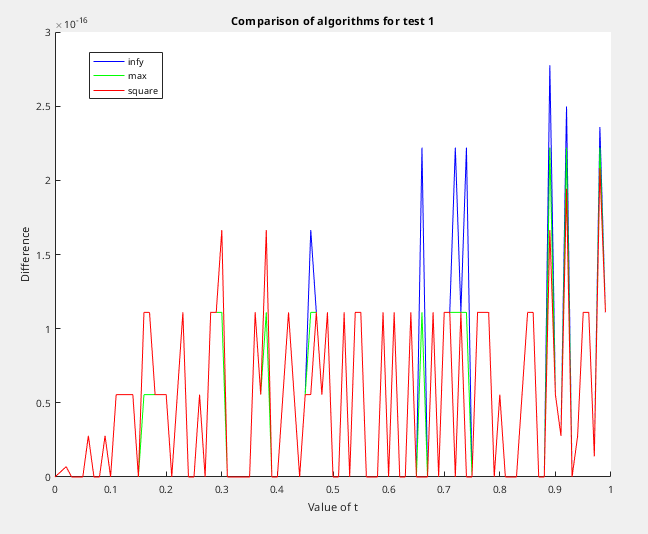
\includegraphics[width=0.8\linewidth]{figs/test01.png}
	\caption{Comparison of algorithms for test 1}
	\label{fig:01}
\end{figure}

\begin{figure}
	\centering
	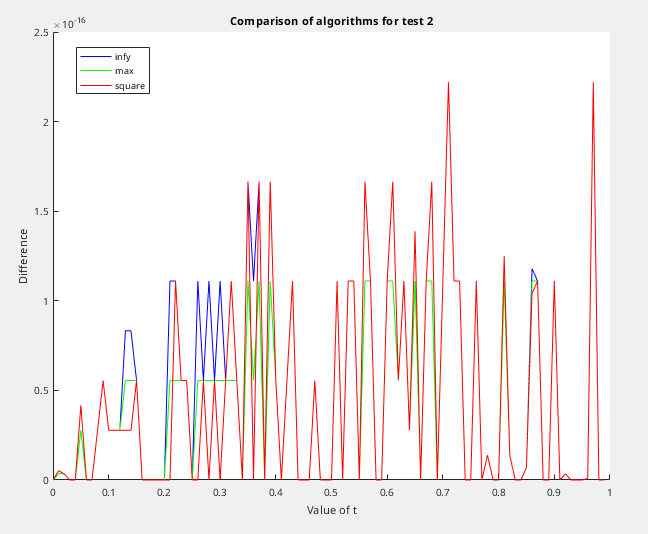
\includegraphics[width=0.8\linewidth]{figs/test02.png}
	\caption{Comparison of algorithms for test 2}
	\label{fig:02}
\end{figure}

\begin{figure}
	\centering
	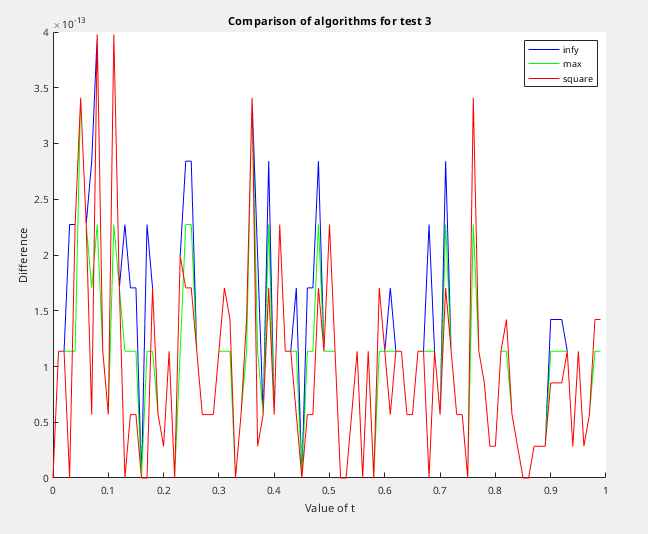
\includegraphics[width=0.8\linewidth]{figs/test03.png}
	\caption{Comparison of algorithms for test 3}
	\label{fig:03}
\end{figure}

\begin{figure}
	\centering
	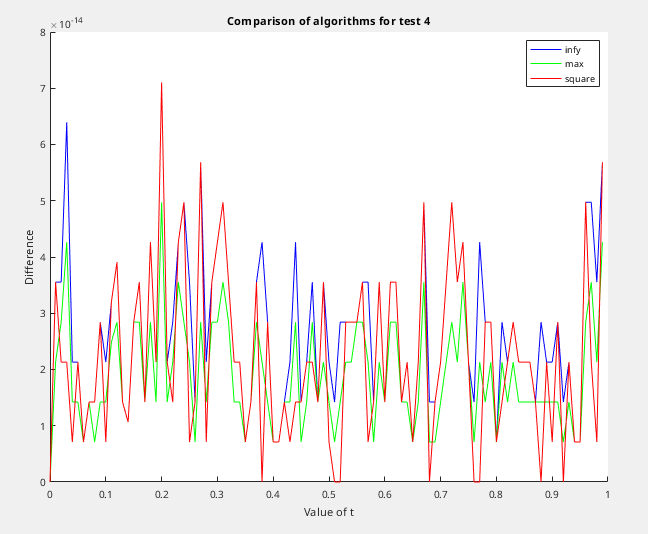
\includegraphics[width=0.8\linewidth]{figs/test04.png}
	\caption{Comparison of algorithms for test 4}
	\label{fig:04}
\end{figure}

\begin{figure}
	\centering
	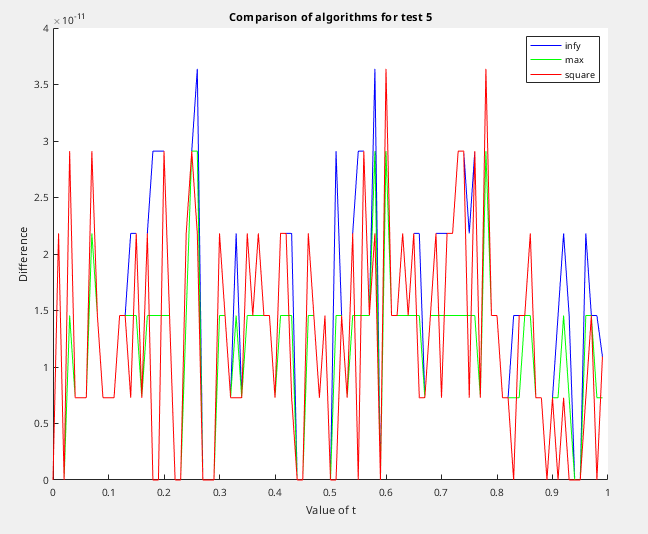
\includegraphics[width=0.8\linewidth]{figs/test05.png}
	\caption{Comparison of algorithms for test 5}
	\label{fig:05}
\end{figure}



\end{document}

